
\begin{table}[h!]
    \centering
    \begin{tabular}{| >{\centering} m{18mm} | >{\centering}m{24mm} | >{\centering}m{18mm} | >{\centering}m{20mm} | >{\centering}m{20mm} | m{20mm} <{\centering}|}
    \hline
       Strategy & Initial Belief Target Present & Mean TTD & Sample SD[TTD] & False Negative Rate & Proportion Incorrectly Localised \\
        \hline
        $\epsilon$-Greedy & 0.25 & 87.6214 & 30.9801 & 0.487 & 0.009 \\
        $\epsilon$-Greedy & 0.5 & 112.93 & 62.38 & 0.152 & 0.040 \\
        $\epsilon$-Greedy & 0.75  & 114.9276 & 81.9386 & 0.0396 & 0.1346 \\
         \hline
        Sweep & 0.25 & 520.4050 & 212.5122 & 0.4292 & 0.0118 \\
        Sweep & 0.5 & 601.57 & 183.45& 0.1254 & 0.0454 \\
        Sweep & 0.75 & 485.3650 & 242.1377 & 0.0326 & 0.1586 \\
        \hline
        Saccadic & 0.25 & 75.8320 & 29.8345 & 0.5054 & 0.0064 \\
        Saccadic & 0.5 & 98.83 & 56.13 & 0.1588 & 0.037 \\
        Saccadic & 0.75 & 100.1332 & 74.3883 & 0.0392 & 0.1418 \\
        \hline
        Random & 0.25 & 539.3802 & 267.6280 & 0.4284 & 0.0074 \\
        Random & 0.5 & 629.55 & 282.95 & 0.137 & 0.0336 \\
        Random & 0.75 & 538.0904 & 325.6283 & 0.035 & 0.1538 \\

    \hline
    \end{tabular}

  \caption{Results of running the target localisation simulation with a varying cumulative  initial belief that the target is present in the search region.}\label{table:VaryingInitialBelief}
\end{table}

\begin{figure}
\centering
    \subfloat[Belief for sweep search prematurely drops below threshold]{{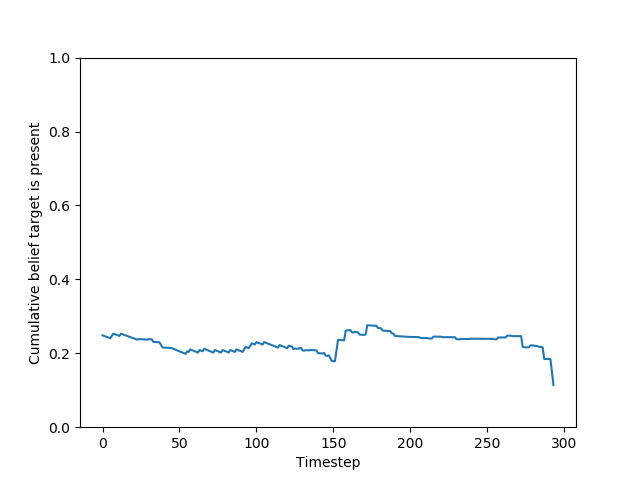
\includegraphics[width=6cm]{Chapters/MultiAgentTargetDetection/Figs/Results/BeliefEvolution/Sweep25InitialBelief/BeliefEvolution1.png} }}%
    \qquad
    \subfloat[Belief for sweep search does not prematurely drop below threshold]{{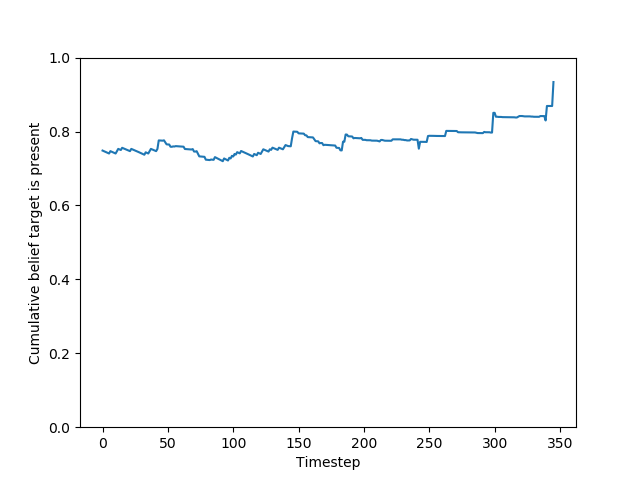
\includegraphics[width=6cm]{Chapters/MultiAgentTargetDetection/Figs/Results/BeliefEvolution/Sweep25InitialBelief/BeliefEvolution4.png} }}%
    \caption{Initial belief distributions}%
    \label{fig:initialCumulativeBelief}%
\end{figure}

Table \ref{table:VaryingInitialBelief} displays the results of running a simulation with a single agent and a single target while varying the agent's cumulative initial belief that the target is present in the search region. We discuss the results in relation to the adaptive and non-adaptive search methods:
\begin{itemize}
    \item The results show that for the non-adaptive Sweep and Random search strategies, the mean TTD decreases when the initial belief that the target is present is set to 0.25 or 0.75. In the case of the 0.25 initial belief value, the lower bound on the observations is found to be 62 consecutive negative observations at distinct locations for the SPRT to determine the target is not present. It is not likely for this to happen for the given parameters, but there are much more likely scenarios that occur which cause the search to terminate early, for example observing 88 negative observations and 16 positive observations.
    %or 1 positive observation and 71 negative observations at distinct locations to pass the threshold(in the absence of any positive observations). Since there are 100 possible starting locations for the source, this is a likely scenario and
    The search terminates prematurely in a high proportion of cases, before a significant number of positive observations are observed to move the cumulative belief of the target presence away from the lower decision boundary. This can be observed in Figure \ref{fig:initialCumulativeBelief}, where on the left hand side there are not a sufficient number of positive observations to stop the search from terminating early. In the case of the 0.75 initial belief value, fewer positive observations are required to reach the upper termination criteria set by the SPRT compared to starting with an initial belief of 0.5, with the same phenomena occurring for the belief starting at 0.25. In the best case, a starting belief of 0.25 would need 6 consecutive positive observations at the same location to cross the upper termination threshold, whereas a starting belief of 0.5 would  require 5 and a starting belief of 0.75 would only require 4. This comes at the price of making it easier to incorrectly identify the target location, increasing the proportion of runs where the target is incorrectly localised. 
    
    \item The mean TTD only decreases for the non-adaptive $\epsilon$-greedy and Saccadic search methods in the case that the initial belief is 0.25 and slightly goes up for both in the case where it is 0.75. We had expected the mean time to decision to decrease in the case of the initial belief starting at 0.75 and increase in the case of the initial belief starting at 0.25, since they are respectively closer and further away from the upper SPRT decision boundary.
    %, due to the fact that it should require more samples to reach a positive conclusion. 
    The reason for the reduced mean TTD with an initial belief of 0.25 for the adaptive search methods is the same as that for the non-adaptive search methods, where the relatively large number of negative samples drove the cumulative belief below the SPRT threshold prematurely. The answer to the question of why the mean time to decision is less than that for the non-adaptive search methods can be explained by the biased sampling nature of the adaptive methods. If one of the adaptive methods comes across a spurious positive, the next choice of sample location will be the same (or probably be the same in the $\epsilon$-greedy case). For the parameters in this run of the simulation, after one positive spurious observation and one subsequent negative observation in the same location, the agent's belief that the target is present would be 0.2496. For the same scenario in the non-adaptive case, the agent would not re-sample the location with the spurious positive observation, but would continue on to sample the next location, which is likely to be a negative observation. In this case, the agent's belief that the target is present would be 0.2545, which is significantly higher than the adaptive case. Since the adaptive agent will re-sample spurious positives, it is able to then rule them out more quickly as potential target locations and as a result the expected time to decision is much lower than that for the non-adaptive methods. The slight increase in the TTD in the case where the initial belief is set to 0.75 is due to the large number of samples needed to break the lower threshold for the SPRT. For the cases where the initial belief set to 0.5 and 0.75, five and four consecutive positive observations at the same location are needed to cross the upper threshold respectively. 139 consecutive negative observations (100 at distinct locations, 39 at previously observed locations) would be needed to cross the lower threshold in the case of starting with an initial cumulative belief of 0.5 whereas 200 consecutive negative observations (100 distinct locations with 2 observations each) would be needed to cross the lower threshold in the case of starting with an initial cumulative belief of 0.75. The mean time to reach a negative decision was 309.1111 and 293.7143 for the $\epsilon$-greedy and saccadic cases with initial belief 0.75, compared to 196.6622 and 177.3552 with initial belief 0.5. The mean time to reach a positive decision was 106.9209 and 92.2352 for the $\epsilon$-greedy and saccadic cases with initial belief 0.75, compared to 97.9630 and 84.0031 with initial belief 0.5. 
    %The significantly longer time needed to reach a negative conclusion accounts for the slightly longer time to reach a decision when the initial belief is set to 0.5.
\end{itemize}


%Really what want to say is that it takes 4 positive obs in same location to reach a decision and mean ttd for e greedy, saccadic are 97.96298915605847/196.6622691292876 and 84.00309082263433/177.3551637279597 with init 0.5 compared to 106.92086630570596/309.1111111111111 and 92.23522064945878/293.7142857142857









